%%%%%%%%%%%%%%%%%%%%%%%%%%%%%%%%%%%%%%%%%%%%%%%%%%%%%%%%%%%
\subsection{Apply statistical model to data}
%%%%%%%%%%%%%%%%%%%%%%%%%%%%%%%%%%%%%%%%%%%%%%%%%%%%%%%%%%%
%
%
\begin{frame}[t, negative]
	\subsectionpage
\end{frame}
%
%
\begin{frame}
	{What we have so far}
	%
	\begin{columns}
		%
		\begin{column}{0.5\textwidth}
			%
			\begin{enumerate}
				%
				\item measure: \\
				replicated entropies $H^{O}_{ik}$
				%
				\item estimand: \\
				$SI$ index, $SEM$ parameters, contrasts
				%
				\item structural models: \\
				total and direct effects
				%
				\item probabilistic models: \\
				three possible fitting models
				%
				\item statistical models: \\
				works as intended
				%
				\item power: \\
				enough
				%
				\item model to data: \\
				\textcolor{blue}{to select the most fitting model}
				%
			\end{enumerate}
			%
		\end{column}
		%
		\begin{column}{0.5\textwidth}  
			%
			Point $7$ uses \\
			Information Theoretic Approach \cite{Anderson_2008, Chamberlain_1965}
			%
			\begin{enumerate}
				%
				\item \sout{hypothesis into statistical models},
				\item select among competing models, 
				\item make inferences based on one or multiple models.
				%
			\end{enumerate}
			
			We select models according to information criteria,
			%
			\begin{enumerate}
				%
				\item WAIC \cite{Watanabe_2013}
				\item PSIS \cite{Vehtari_et_al_2021}
				%
			\end{enumerate}
			%
		\end{column}
		%
	\end{columns}
	%
\end{frame}
%
%
\begin{lhframe}[rhgraphic={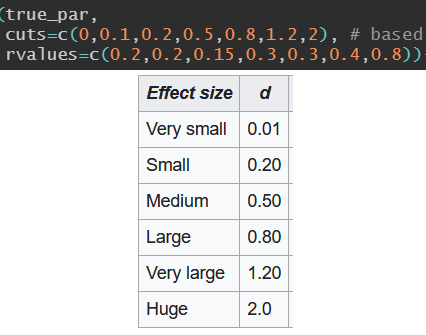
\includegraphics[scale=0.40]{ES_ROPE.png}}]
	{Competing models}
	%
	
	%
\end{lhframe}
%
%
